% Load paths on a blade, its hub and a motor arm (README Figure 4).
% Compile: pdflatex load_paths.tex   (needs stanli, TikZ; MiKTeX installs them on demand)
\documentclass[tikz,border=8pt]{standalone}
\usepackage{amsmath}
\usepackage{stanli}
\usetikzlibrary{arrows.meta,calc,patterns,decorations.pathmorphing,positioning}

% Okabe-Ito colour-blind-safe palette
\definecolor{cbblue}{HTML}{0072B2}
\definecolor{cbred}{HTML}{D55E00}
\definecolor{cbgreen}{HTML}{009E73}
\definecolor{cborange}{HTML}{E69F00}
\definecolor{cbpurple}{HTML}{CC79A7}
\definecolor{cbgrey}{HTML}{555555}

\tikzset{
  force/.style={-{Stealth[length=2.6mm]}, line width=1.2pt},
  comp/.style={-{Stealth[length=2mm]}, line width=0.9pt, dash pattern=on 3pt off 2pt},
  lab/.style={font=\small, inner sep=1.5pt},
  panel/.style={font=\small, anchor=west},
  blade/.style={draw=cbblue, fill=cbblue!12, line width=0.9pt},
  wall/.style={draw=black, pattern=north east lines, pattern color=cbgrey},
}

\begin{document}
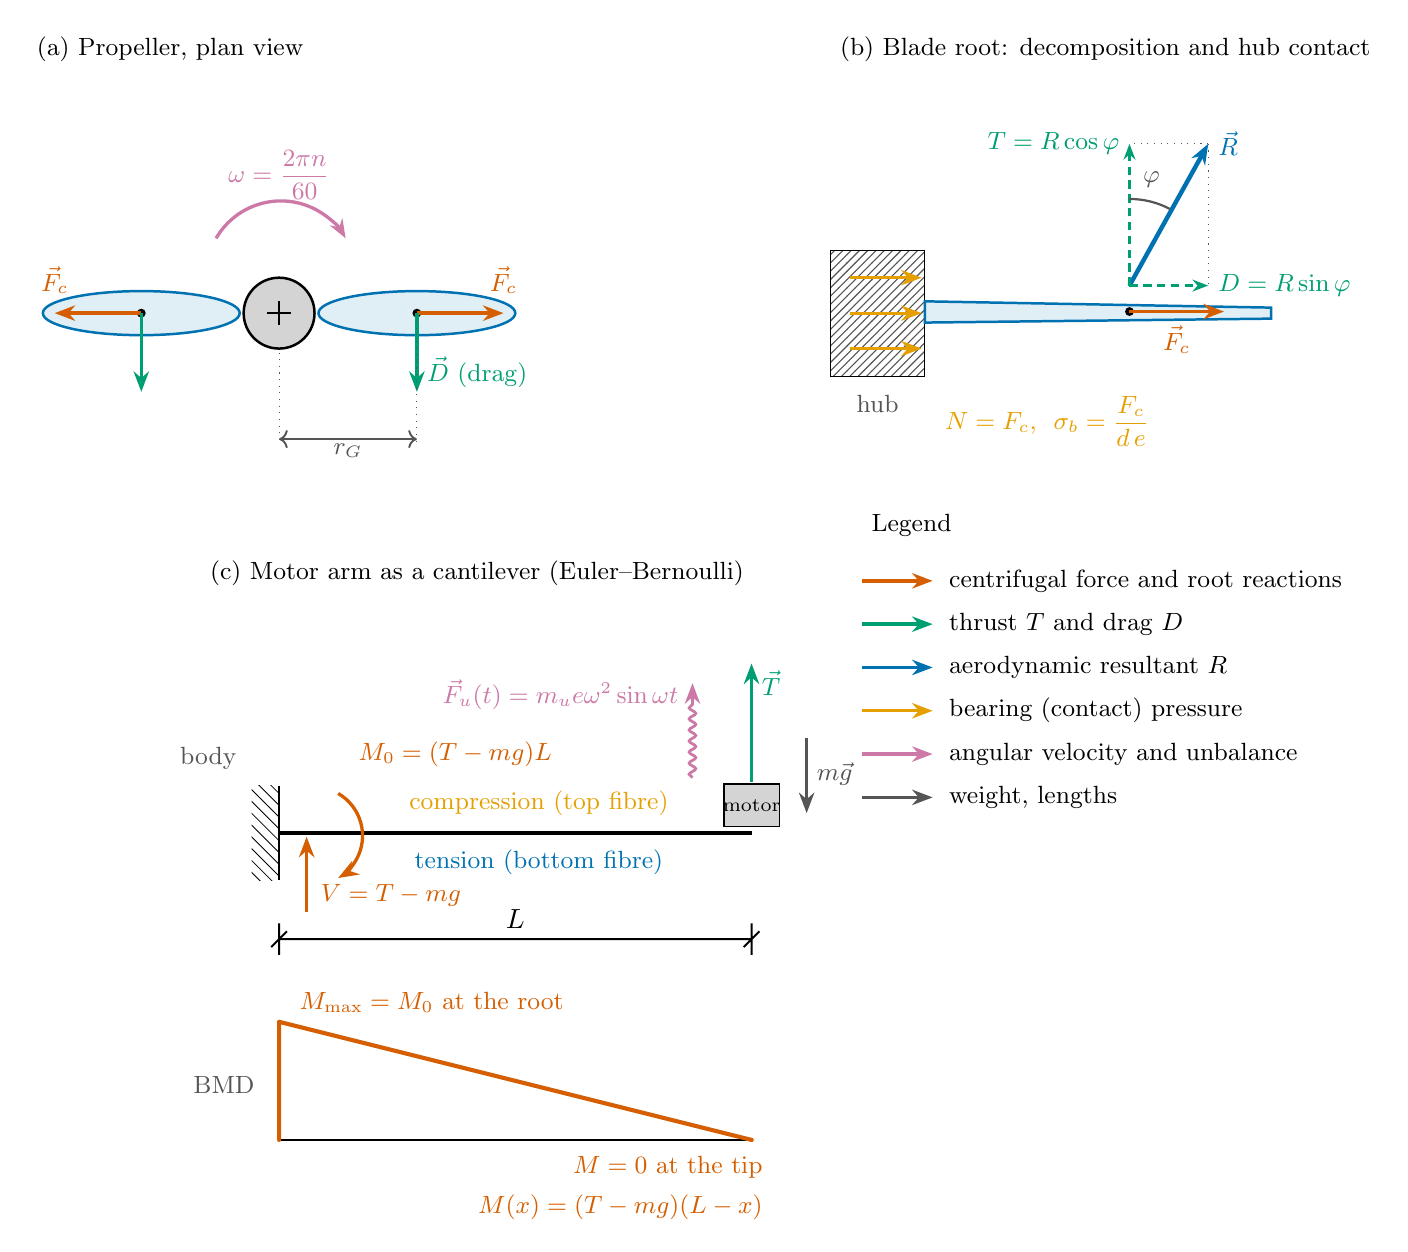
\begin{tikzpicture}

%% (a) propeller, plan view -----------------------------------------------------------------------------
\begin{scope}[shift={(0,0)}]
  \node[panel] at (-3.2,3.35) {(a) Propeller, plan view};
  \draw[blade] (-1.75,0) ellipse (1.25 and 0.28);
  \draw[blade] ( 1.75,0) ellipse (1.25 and 0.28);
  \draw[fill=cbgrey!25, draw=black, line width=0.9pt] (0,0) circle (0.45);
  \draw[line width=0.6pt] (-0.15,0) -- (0.15,0) (0,-0.15) -- (0,0.15);
  % centre of mass of each blade, centrifugal force and drag
  \foreach \s in {-1,1}{
    \fill (\s*1.75,0) circle (1.6pt);
    \draw[force, cbred]   (\s*1.75,0) -- ++(\s*1.1,0);
    \draw[force, cbgreen] (\s*1.75,0) -- ++(0,-1.0);
  }
  \node[lab, cbred, above=3pt]  at (2.85,0.08) {$\vec F_c$};
  \node[lab, cbred, above=3pt]  at (-2.85,0.08) {$\vec F_c$};
  \node[lab, cbgreen, right=2pt] at (1.75,-0.75) {$\vec D$ (drag)};
  % angular velocity
  \draw[-{Stealth[length=2.4mm]}, cbpurple, line width=1.2pt] (-0.8,0.95) arc[start angle=150, end angle=30, radius=0.95];
  \node[lab, cbpurple] at (0,1.75) {$\omega=\dfrac{2\pi n}{60}$};
  % lever arm r_G
  \draw[<->, cbgrey, line width=0.7pt] (0,-1.6) -- node[below, lab, text=cbgrey] {$r_G$} (1.75,-1.6);
  \draw[cbgrey, dotted] (0,-0.5) -- (0,-1.65) (1.75,-0.1) -- (1.75,-1.65);
\end{scope}

%% (b) blade root: decomposition and hub contact -------------------------------------------------------
\begin{scope}[shift={(8.2,0)}]
  \node[panel] at (-1.2,3.35) {(b) Blade root: decomposition and hub contact};
  \draw[wall] (-1.2,-0.8) rectangle (0,0.8);
  \node[lab, text=cbgrey] at (-0.6,-1.15) {hub};
  \draw[blade] (0,-0.12) -- (4.4,-0.07) -- (4.4,0.07) -- (0,0.15) -- cycle;
  \fill (2.6,0.02) circle (1.6pt);
  \draw[force, cbred] (2.6,0.02) -- ++(1.2,0);
  \node[lab, cbred, below=3pt] at (3.2,0) {$\vec F_c$};
  % aerodynamic resultant and its components at the blade
  \coordinate (O) at (2.6,0.35);
  \draw[force, cbblue, line width=1.6pt] (O) -- ++(1.0,1.8) coordinate (Rend);
  \draw[comp, cbgreen] (O) -- ++(0,1.8) coordinate (Tend);
  \draw[comp, cbgreen] (O) -- ++(1.0,0) coordinate (Dend);
  \draw[cbgrey, dotted] (Rend) -- (Tend) (Rend) -- (Dend);
  \node[lab, cbblue, right=2pt] at (Rend) {$\vec R$};
  \node[lab, cbgreen, left=2pt] at (Tend) {$T=R\cos\varphi$};
  \node[lab, cbgreen, right=2pt] at (Dend) {$D=R\sin\varphi$};
  \draw[cbgrey, line width=0.8pt] ($(O)+(0,1.1)$) arc[start angle=90, end angle=62, radius=1.1];
  \node[lab, text=cbgrey] at ($(O)+(0.28,1.35)$) {$\varphi$};
  % bearing (contact) pressure at the hub face
  \foreach \y in {-0.45,0,0.45}{ \draw[force, cborange, line width=1pt] (-0.95,\y) -- (-0.04,\y); }
  \node[lab, cborange, anchor=north west, align=left] at (0.2,-1.0) {$N=F_c$,\ \ $\sigma_b=\dfrac{F_c}{d\,e}$};
\end{scope}

%% (c) motor arm as a cantilever ---------------------------------------------------------------------
\begin{scope}[shift={(0,-6.6)}]
  \node[panel] at (-1.0,3.3) {(c) Motor arm as a cantilever (Euler--Bernoulli)};
  \point{a}{0}{0}\point{b}{6}{0}
  \beam{2}{a}{b}
  \support{3}{a}[-90]
  \node[lab, text=cbgrey] at (-0.9,0.95) {body};
  % motor at the tip and loads
  \draw[fill=cbgrey!25, draw=black] (5.65,0.08) rectangle (6.35,0.62);
  \node[font=\scriptsize] at (6.0,0.35) {motor};
  \draw[force, cbgreen] (6.0,0.65) -- ++(0,1.5);
  \node[lab, cbgreen, right=2pt] at (6.0,1.9) {$\vec T$};
  \draw[force, cbgrey] (6.7,1.2) -- ++(0,-0.95);
  \node[lab, cbgrey, right=2pt] at (6.7,0.75) {$m\vec g$};
  % rotating unbalance (zig-zag with arrow)
  \draw[decorate, decoration={snake, amplitude=1.2pt, segment length=4pt}, cbpurple, line width=1pt] (5.25,0.7) -- ++(0,1.0);
  \draw[force, cbpurple] (5.25,1.7) -- ++(0,0.2);
  \node[lab, cbpurple, left=2pt, align=right] at (5.2,1.75) {$\vec F_u(t)=m_ue\omega^{2}\sin\omega t$};
  % reactions at the root
  \draw[force, cbred] (0.35,-1.0) -- ++(0,0.95);
  \node[lab, cbred, right=2pt] at (0.4,-0.8) {$V=T-mg$};
  \draw[force, cbred] (0.75,0.5) arc[start angle=60, end angle=-60, radius=0.62] ;
  \node[lab, cbred, anchor=west] at (0.95,1.0) {$M_0=(T-mg)L$};
  % stress state
  \node[lab, text=cborange] at (3.3,0.38) {compression (top fibre)};
  \node[lab, text=cbblue] at (3.3,-0.38) {tension (bottom fibre)};
  \dimensioning{1}{a}{b}{-1.35}[$L$]
  % bending-moment diagram
  \point{c}{0}{-3.9}\point{d}{6}{-3.9}
  \draw[line width=0.8pt] (c) -- (d);
  \internalforces{c}{d}{-1.5}{0}[0][cbred]
  \node[lab, cbred, anchor=west] at (0.2,-2.15) {$M_{\max}=M_0$ at the root};
  \node[lab, cbred, anchor=east] at (6.2,-4.25) {$M=0$ at the tip};
  \node[lab, cbred, anchor=east] at (6.2,-4.75) {$M(x)=(T-mg)(L-x)$};
  \node[lab, text=cbgrey] at (-0.7,-3.2) {BMD};
\end{scope}

%% (d) legend of the vector colours ---------------------------------------------------------------
\begin{scope}[shift={(8.6,-4.6)}]
  \node[panel] at (-1.2,1.9) {Legend};
  \foreach \c/\t [count=\i from 0] in {cbred/{centrifugal force and root reactions},
       cbgreen/{thrust $T$ and drag $D$}, cbblue/{aerodynamic resultant $R$},
       cborange/{bearing (contact) pressure}, cbpurple/{angular velocity and unbalance}, cbgrey/{weight, lengths}}{
    \draw[force, \c] (-1.2,1.2-0.55*\i) -- ++(0.9,0);
    \node[lab, anchor=west] at (-0.15,1.2-0.55*\i) {\t};
  }
\end{scope}

\end{tikzpicture}
\end{document}
